\chapter{Integration Techniques}
\section{Basic Integration (IBS, IBP, etc)}
\begin{stbox}{General Information}
  \begin{enumerate}
    \item Factor Formulae (remember these):
    \begin{enumerate}
      \item \(\sin(mx)\cos(nx)=\frac{1}{2}[\sin((m+n)x)+\sin((m-n)x)]\),
      \item \(\cos(mx)\cos(nx)=\frac{1}{2}[\cos((m+n)x)+\cos((m-n)x)]\),
      \item \(\sin(mx)\sin(nx)=-\frac{1}{2}[\cos((m+n)x)-\cos((m-n)x)]\).
    \end{enumerate}
    \item Common classes of integrals:
    \begin{enumerate}
      \item Apply partial fractions:
      \[\int\frac{f(x)}{g(x)}\,dx.\]
      \item Split \(px+q\), then complete the square:
      \[\int \frac{px+q}{\sqrt{ax^2+bx+c}}\,dx \quad\text{or}\quad \int \frac{px+q}{ax^2+bx+c}\,dx\] 
    \end{enumerate}
    \item Partial fractions. First ensure the numerator has a smaller degree than that of the denominator, otherwise do long division first. Then,
    \begin{flalign*}
      \text{(i)}\quad &\frac{P(x)}{(ax+b)(cx+d)}=\frac{A}{ax+b}+\frac{B}{cx+d}\\
      \text{(ii)}\quad &\frac{P(x)}{(ax+b)^2}=\frac{A}{ax+b}+\frac{B}{(ax+b)^2}\\
      \text{(iii)}\quad &\frac{P(x)}{(ax+b)(cx^2+dx+e)}=\frac{A}{ax+b}+\frac{Bx+C}{cx^2+de+e}
    \end{flalign*}
    where \(cx^2+de+e\) is irreducible, i.e. has non-real roots.
    \item Integration by Substitution: 
    \[\int f(x) \, dx=\int f(x)\frac{dx}{du}\,du.\]
    \item Use Pythagoras' Theorem / draw a right-angled triangle to help with trig conversions, e.g.:
    \[\tan(\theta) \qquad\text{to}\qquad \frac{x+1}{\sqrt{2-(x+1)^2}}.\]
    \item Integration by Parts:

    \begin{minipage}{0.5\textwidth-12.5pt}
      \begin{alignat*}{3}
        &\text{Let }& u&=\rule{0.5cm}{0.01mm} &\qquad  v&=\rule{0.5cm}{0.01mm}\\
        &&\dfrac{du}{dx} &=\rule{0.5cm}{0.01mm} & \dfrac{dv}{dx}&=\rule{0.5cm}{0.01mm}
       \end{alignat*} 
    \end{minipage}%
    \begin{minipage}{0.5\textwidth-12.5pt}
      \[\int u\left(\frac{dv}{dx}\right)\,dx=uv-\int v \left(\frac{du}{dx}\right)\,dx.\]
    \end{minipage}
  \end{enumerate}
\end{stbox}
\section{Areas \& Volumes}
\begin{figure}[H]
  \centering
  \begin{subfigure}{0.9\textwidth}
    \centering
    \includegraphics[width=\textwidth,page=1]{../Diagrams/disc-method/diagram2.pdf}

    \includegraphics[width=\textwidth,page=2]{../Diagrams/disc-method/diagram2.pdf}
    \caption{\(y=\sqrt{x}\)}
    \label{fig:disc-quadratic}
\end{subfigure}%

\begin{subfigure}{0.9\textwidth}
    \centering
    \includegraphics[width=\textwidth,page=3]{../Diagrams/disc-method/diagram2.pdf}

    \includegraphics[width=\textwidth,page=4]{../Diagrams/disc-method/diagram2.pdf}
    \caption{\(y=2e^{-x/2}\)}
    \label{fig:disc-func}
\end{subfigure}
  \caption{\ref{source:disc} The disc method.}
  \label{fig:disc}
\end{figure}
\begin{figure}[H]
  \centering
  \includegraphics{../Diagrams/shell-method/diagram1.pdf}
  \caption{\ref{source:shell} The shell method.}
  \label{fig:shell}
\end{figure}
\begin{stbox}{General Information}
  \begin{enumerate}
    \item Volume of revolution when rotated about \(x\)-axis: 
  \begin{enumerate}
    \item The disc method (Figure \ref{fig:disc}):
    \[\int_{x_1}^{x_2}\pi y^2\,dx=\int_{x=x_1}^{x=x_2}\pi y^2\, \frac{dx}{dt}\,dt.\]
    \item The shell method (Figure \ref{fig:shell}):
    \[\int_{y_1}^{y_2}2\pi yx \,dy.\]
  \end{enumerate}
  \item Arc length:
  \begin{equation*}
    \resizebox{0.9\hsize}{!}{\(\displaystyle\int_{x_1}^{x_2}\sqrt{\left(\frac{dy}{dx}\right)^2+1}\,dx=\int_{y_1}^{y_2} \sqrt{\left(\frac{dx}{dy}\right)^2+1}\,dy=\int_{t_1}^{t_2}\sqrt{\left(\frac{dy}{dt}\right)^2+\left(\frac{dx}{dt}\right)^2}\,dt=\int_{\alpha}^{\beta}\sqrt{r^2+\left(\frac{dr}{d\theta}\right)^2}\,d\theta.\)}
    \end{equation*}
  \item Surface area of revolution when rotated about \(\highlight[blue!30]{x}\)-axis: 
  \begin{equation*}
    \resizebox{0.9\hsize}{!}{\(\displaystyle\int_{x_1}^{x_2}2\pi \highlight[red!30]{y} \sqrt{\left(\frac{dy}{dx}\right)^2+1}\,dx=\int_{y_1}^{y_2}2\pi \highlight[red!30]{y} \sqrt{\left(\frac{dx}{dy}\right)^2+1}\,dy=\int_{t_1}^{t_2}2\pi \highlight[red!30]{y} \sqrt{\left(\frac{dy}{dt}\right)^2+\left(\frac{dx}{dt}\right)^2}\,dt.\)}
    \end{equation*}
  \begin{flushleft}
    \(\bigstar\) Rotating about \(\highlight[blue!30]{x}\)-axis \(\implies\) \(\highlight[red!30]{y}\) in integrand\\
    \hphantom{\(\bigstar\)} Rotating about \(\highlight[blue!30]{y}\)-axis \(\implies\) \(\highlight[red!30]{x}\) in integrand.
  \end{flushleft}
  \item Area enclosed by a polar curve:
  \[\int_{\alpha}^{\beta}\frac{1}{2}r^2\,d\theta.\]
  \end{enumerate}
\end{stbox}
\begin{example}{Geometrical interpretation of an approximate area}{}
  An parabolic arc has equation \(x=at^2\), \(y=2at\) for \(0\leq t\leq p\). When rotated through \(2\pi\) radians about the \(x\)-axis, the surface area of revolution formed is \(A=8\pi a^2/3\left[ (p^2+1)^{3/2}-1 \right]\) units\(^2\). Consider the approximation to \(A\) when \(p\) is sufficiently small, such that powers above \(p^2\) can be ignored. Interpret this approximate area geometrically.
  \[A\approx 8/3\pi a^2[1+3/2p^2-1]=4\pi a^2p^2\text{ units}^2\ (=\pi(2ap)(2ap)).\]
  Geometric interpretation: The approximate area is the surface area of a cone with radius \(2ap\) and approximate slant height \(2ap\). 
  \begin{figure}[H]
    \centering
    \begin{subfigure}{0.475\textwidth}
      \centering
      \includegraphics[width=\textwidth]{../Diagrams/approximate-surface-area/curve.pdf}
      \caption{2d illustration.}
  \end{subfigure}\hfill
  \begin{subfigure}{0.475\textwidth}
      \centering
      \includegraphics[width=\textwidth]{../Diagrams/approximate-surface-area/3d.pdf}
      \caption{3d illustration.}
  \end{subfigure}
    \caption{\ref{Me}}
    \label{fig:surface-area}
  \end{figure}
  \emph{Note.} The slant height \(\ell=\sqrt{(ap^2)^2+(2ap)^2}=\sqrt{a^2p^4+4a^2p^2}\approx\sqrt{a^2\cdot 0+4a^2p^2}=2ap\).
\end{example}
\section{Numerical Methods}
\subsection{Trapezium Rule}
\begin{stbox}{General Information}
    \begin{enumerate}
      \item Formula for \(n\) intervals, or (n+1)ordinates, of width \(h\coloneq (b-a)/n\): 
      \[\int_{a}^{b}y\,dx=\frac{h}{2}(y_0+2y_1+2y_2+\cdots+2y_{n-1}+y_n).\]
      \item Illustration
      \begin{figure}[H]
        \centering
        \includestandalone{../Diagrams/Trapezium}
        \caption{\ref{source:trapzium-rule} Trapezium rule.}
        \label{fig:trapzium-rule}
      \end{figure}
    \item Error: 
    \begin{enumerate}
      \item Concave upwards, i.e. (\(f'(x)\) is increasing / \(f''(x)>0\)) \(\implies\) overestimation.
      \item Concave downwards, i.e. (\(f'(x)\) is decreasing / \(f''(x)<0\)) \(\implies\) underestimation.
    \end{enumerate}
    \end{enumerate}
    \end{stbox}
    \begin{note}
      State and explain whether the trapezium rule gives an underestimate or an overestimate of the area of under the curve \(y=f(x)\) from \(x=x_0\) to \(x=x_1\).
      \begin{figure}[H]
        \centering
        \includegraphics[width=0.4\textwidth]{../Diagrams/trapzium-estimate.pdf}
        \caption{\ref{source:trapzium-rule} The trapezium rule results in an overestimate for the area under a curve that is concave upwards.}
        \label{fig:trapezium-overestimate}
      \end{figure}
      From the diagram and the fact that \(\frac{d^2y}{dx^2}=\rule{0.5cm}{0.01mm}>0\) for all \(x\in[a,b]\), the curve is concave upwards. As such, the trapeziums contain the graph of \(y=f(x)\), for \(x\in[a,b]\). So, the trapezium rule gives a overestimate.
    \end{note}
    \subsection{Simpson's Rule}
    \begin{stbox}{General Information}
      \begin{enumerate}
        \item Formula for \(n\) intervals, or (n+1)ordinates, of width \(h\coloneq (b-a)/n\):
        \[\int_{a}^{b}y\,dx=\frac{h}{3}(y_0+4y_1+2y_2+4y_3+\cdots+2y_{n-2}+4y_{n-1}+y_n).\]
        Note that the number of intervals \(n\) should be \emph{even}, that of ordinates \emph{odd}.
        \item Illustration
        \begin{figure}[H]
          \centering
          \includestandalone{../Diagrams/Simpson}
          \caption{\ref{source:simpson's-rule} Simpson's rule.}
          \label{fig:simpson's-rule}
        \end{figure}
        \item Simpson's Rule is exact for all polynomials of degree three and below.
      \end{enumerate}
    \end{stbox}
    \begin{example}{}{}
      Explain, with the aid of a suitable diagram, why Simpson's Rule does not give a good approximation of the value of \(I=\int_{a}^{b}f(x)\,dx\) and suggest how the method can be improved to give a better approximation.

      \rule{20cm-137.0549pt-25pt}{0.05mm}

      \begin{figure}[H]
        \centering
        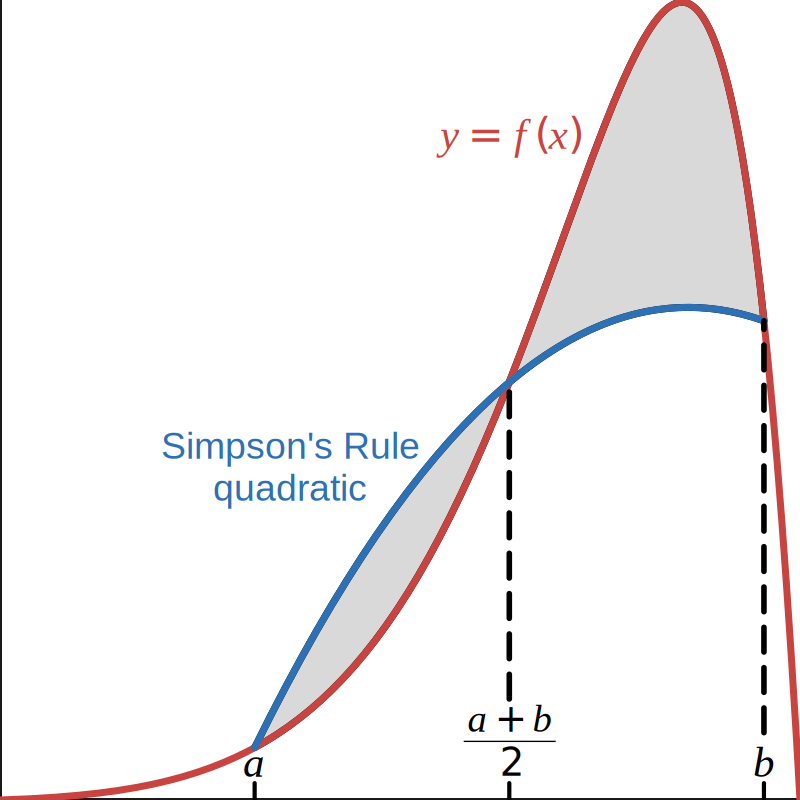
\includegraphics[width=0.425\textwidth]{../Diagrams/simpson-underestimate.pdf}
        \caption{\ref{Me} \href{https://www.desmos.com/calculator/wxxs9ypjkf}{(Desmos)}}
        \label{fig:simpson's-rule-overestimate-prelims}
      \end{figure}
      We see that there is a large discrepancy between the area under the actual curve \(y=f(x)\) and the approximated quadratic curve for the interval \(a\leq x\leq b\), which is caused by [the existence of both a turning point and a point of inflection]. Hence, Simpson's Rule using \(n\) ordinates will not provide a good approximation in this case.
    \end{example}
    \begin{note}
      Accuracy of the Trapezium rule vs Simpson's Rule:
      ``Simpson's Rule uses \emph{quadratic curves} to interpolate the points on the curve so it usually \emph{gives a better approximation} to the actual curve than the trapezium rule which uses \emph{straight lines} to interpolate the ordinates.''
    \end{note}
\section{Reduction formulas}
\begin{stbox}{General Information}{}
  Let \(I_n\coloneq\int_{a}^{b}f(x)\,dx\). To find a reduction formula for \(I_n\), we use integration by parts on \(I_n\).

  \emph{Note.} Integrating \(I_{n-1},I_{n+1},\text{etc}\) (by parts) typically does not produce nice results.  
\end{stbox}
Sometimes, some algebraic tricks are needed to reduce an integral into the desired form. Try to spot these, before attempting another round of integration by parts. 
\begin{example}{Rewriting \(x^2\) as \((4-x^2)-4\)}{}
  % \begin{alignat*}{3}
  %   &\text{Let }& u&=\dfrac{1}{(4-x^2)^n} &\qquad  v&=1\\
  %   &&\dfrac{du}{dx} &=\dfrac{2nx}{(4-x^2)^{n+1}} & \dfrac{dv}{dx}&=x
  %  \end{alignat*}
  Using
   \begin{alignat*}{2}
    u&=\dfrac{1}{(4-x^2)^n} &\qquad  v&=1\\
    \dfrac{du}{dx} &=\dfrac{2nx}{(4-x^2)^{n+1}} & \dfrac{dv}{dx}&=x
   \end{alignat*}
   we evaluate \(A_n\coloneq\int_{0}^{1/2}\frac{1}{(4-x^2)^n}\,dx\):
{\allowdisplaybreaks
     \begin{align*}
    A_n&=\frac{1}{2}{\left( \frac{4}{15} \right)^n}-2n\int_{0}^{1/2}\frac{x^2}{(4-x^2)^{n+1}}\,dx\\
    &=\frac{1}{2}{\left( \frac{4}{15} \right)^n}+2n\int_{0}^{1/2}\frac{\highlight[yellow]{(4-x^2)-4}}{(4-x^2)^{n+1}}\,dx\\
    &=\frac{1}{2}{\left( \frac{4}{15} \right)^n}+2n\int_{0}^{1/2}\frac{4-x^2}{(4-x^2)^n}-4\cdot\frac{1}{(4-x^2)^{n+1}}\,dx\\
    &=\frac{1}{2}{\left( \frac{4}{15} \right)^n}+2n(A_n-4A_{n+1}).\\
   \end{align*}}
   Therefore, \((2n-1)A_n+1/2(4/15)^n=8nA_{n+1}\).
\end{example}